\apendice{Plan de Proyecto Software}

\section{Introducción}
Este apéndice explica la estrategia de gestión 
que ha guiado el ciclo de vida del desarrollo 
del asistente SugAIr. Para ello, se describe en 
primer lugar la organización temporal de las 
tareas y el seguimiento del progreso mediante 
metodologías ágiles. Asimismo, se incluye un 
análisis de la viabilidad del proyecto, 
evaluando tanto la inversión económica teórica 
necesaria para su ejecución como el marco 
normativo y legal que regula el despliegue y el 
tratamiento de los datos en la aplicación.

\section{Planificación temporal}

En el proyecto se han usado metodologías ágiles. Se han utilizado ciclos de desarrollo iterativos (\textit{sprints}) de 3 semanas de duración a lo largo de un periodo de 4 meses.
Para la gestión visual del flujo de trabajo, se ha utilizado un tablero Kanban alojado en GitLab, dividiendo los requisitos en tareas (\textit{issues}). 

\clearpage
\begin{sidewaysfigure}
    \centering
    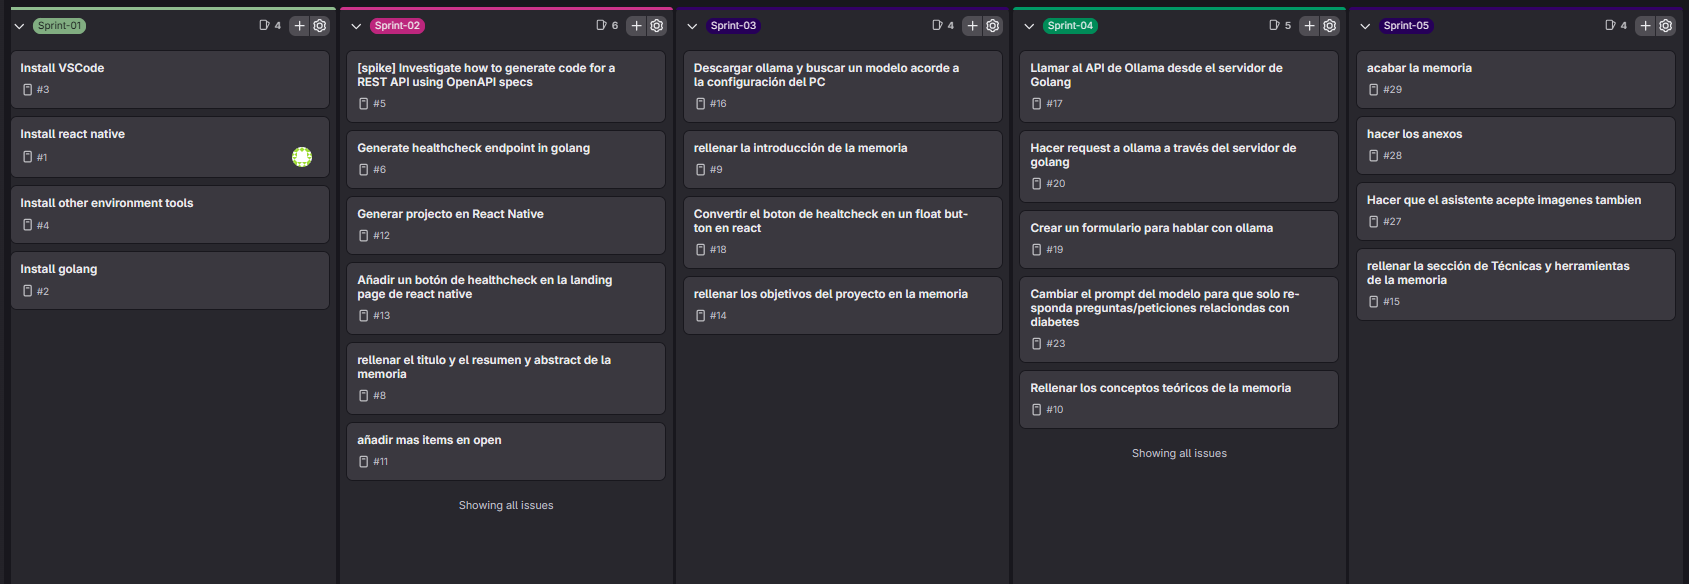
\includegraphics[width=1\linewidth]{tablero_kanban.png}
    \caption{Tablero Kanban de Igor}
    \label{tablero:kanban}
\end{sidewaysfigure}
 Las tareas se definieron y asignaron a cada iteración con el objetivo de garantizar entregas funcionales e incrementales al final de cada \textit{sprint} de 3 semanas.

A continuación, se detalla la evolución del desarrollo a través de los 5 \textit{sprints} realizados:

\subsection*{Sprint 1: Configuración del entorno de desarrollo}
Este primer ciclo abarcó la preparación de la infraestructura de hardware y software necesaria para soportar tanto el desarrollo móvil como el servidor backend.
\begin{itemize}
    \item \textbf{Objetivos técnicos:} Instalación y configuración del entorno de desarrollo integrado (VSCode), el marco de trabajo móvil (React Native), el lenguaje de programación del servidor (Golang) y el resto de dependencias del ecosistema.
\end{itemize}

\subsection*{Sprint 2: Prueba de concepto y API REST base}
El segundo \textit{sprint} se enfocó en establecer el canal de comunicación inicial entre la aplicación móvil y el servidor.
\begin{itemize}
    \item \textbf{Objetivos técnicos:} Investigación (\textit{spike}) sobre la generación de código para APIs REST mediante especificaciones OpenAPI. Creación del proyecto base en React Native y desarrollo de un \textit{endpoint} de comprobación de estado (\textit{healthcheck}) en Golang, verificando la conexión mediante un botón en la \textit{landing page} de la aplicación.
    \item \textbf{Documentación:} Redacción del título, resumen y \textit{abstract} de la memoria.
\end{itemize}

\subsection*{Sprint 3: Interfaz flotante y motor de inferencia local}
Esta iteración abordó dos de los requisitos fundamentales de la app: la ergonomía de la aplicación y la integración del motor de Inteligencia Artificial.
\begin{itemize}
    \item \textbf{Objetivos técnicos:} Descarga, instalación y configuración del entorno Ollama, realizando una búsqueda del modelo de lenguaje local que mejor se ajustase a las especificaciones de hardware del equipo. En el \textit{frontend}, se implementó la lógica para convertir el acceso a la herramienta en un botón flotante (\textit{float button}). Pero en el diseño final se puso otro botón.
    \item \textbf{Documentación:} Redacción de la introducción y los objetivos del proyecto.
\end{itemize}

\subsection*{Sprint 4: Comunicación bidireccional y contexto clínico}
En este ciclo se consolidó el flujo de datos completo, conectando la interfaz del usuario con el modelo de lenguaje.
\begin{itemize}
    \item \textbf{Objetivos técnicos:} Desarrollo de un formulario de chat interactivo en React Native. En el \textit{backend}, se implementaron las peticiones HTTP desde Golang hacia la API local de Ollama. Finalmente, se aplicaron técnicas de ingeniería de contexto (\textit{prompt engineering}) para restringir el modelo, asegurando que las respuestas se limitaran exclusivamente a preguntas relacionadas con la diabetes.
    \item \textbf{Documentación:} Redacción del marco teórico y los conceptos de la memoria.
\end{itemize}

\subsection*{Sprint 5: Integración multimodal y cierre}
El último \textit{sprint} se dedicó a dotar al asistente de capacidades de visión artificial, superando las limitaciones previas, y a la finalización de los entregables académicos.
\begin{itemize}
    \item \textbf{Objetivos técnicos:} Implementación del soporte para el procesamiento de imágenes. Se integró el modelo multimodal Llava y se adaptó el servidor Golang para gestionar y limpiar cadenas de imágenes en formato Base64, permitiendo al usuario adjuntar fotografías al chat (como gráficas de glucosa o etiquetas alimentarias).
    \item \textbf{Documentación:} Redacción del capítulo de técnicas y herramientas, desarrollo de los anexos y revisión final de la memoria.
\end{itemize}

\section{Estudio de viabilidad}

\subsection{Viabilidad económica}
El análisis de la viabilidad económica tiene como objetivo estimar los costes teóricos que supondría el desarrollo y puesta en marcha del proyecto SugAIr en un entorno empresarial real. Para realizar este cálculo, se han considerado los precios de mercado actuales en España y se ha supuesto un escenario de desarrollo de 4 meses de duración con una jornada laboral completa (8 horas diarias).

\subsubsection*{Costes de personal}
El desarrollo ha sido realizado íntegramente por un perfil de Ingeniería Informática Junior. Se toma como referencia un salario bruto anual promedio para este perfil en España de 21.000,00 \euro{} \cite{glassdoor_salary}. Para obtener el coste real para la empresa, es necesario sumar al salario bruto los costes de la Seguridad Social (contingencias comunes, desempleo, formación, etc.), que se estiman aproximadamente en un 32\,\% del salario bruto.

Los cálculos para los 4 meses de desarrollo son los siguientes:
\begin{itemize}
    \item Salario mensual bruto: $21.000,00\,\text{\euro} / 12 = 1.750,00\,\text{\euro/mes}$.
    \item Coste Seguridad Social (32\,\%): $1.750,00\,\text{\euro} \times 0,32 = 560,00\,\text{\euro/mes}$.
    \item Coste mensual total para la empresa: $1.750,00\,\text{\euro} + 560,00\,\text{\euro} = 2.310,00\,\text{\euro/mes}$.
    \item Coste total del proyecto (4 meses): $2.310,00\,\text{\euro} \times 4 = 9.240,00\,\text{\euro}$.
\end{itemize}

\subsubsection*{Costes de hardware}
Para el desarrollo y la compilación de la Inteligencia Artificial local, se ha utilizado un equipo informático portátil (ASUS) con un precio de mercado estimado de 600,00 \euro. El coste imputable al proyecto se calcula mediante la amortización del equipo durante el tiempo de uso (4 meses), estimando una vida útil estándar de 4 años (48 meses).

\begin{itemize}
    \item Amortización mensual: $600,00\,\text{\euro} / 48 = 12,50\,\text{\euro/mes}$.
    \item Coste total hardware (4 meses): $12,50\,\text{\euro} \times 4 = 50,00\,\text{\euro}$.
\end{itemize}

\subsubsection*{Costes de software e infraestructura}
El proyecto SugAIr se ha desarrollado priorizando el uso de tecnologías de código abierto y herramientas gratuitas, lo que reduce drásticamente los costes de licencias. El \textit{stack} tecnológico incluye Go, React Native, Ollama y Visual Studio Code, todos ellos gratuitos. El único coste de software imputable corresponde a una licencia comercial de Microsoft Windows 10, con un precio aproximado de 145,00 \euro, amortizada a 4 años ($3,02\,\text{\euro/mes} \times 4 = 12,08\,\text{\euro}$).

En cuanto a los costes de infraestructura, el diseño arquitectónico de SugAIr presenta una ventaja competitiva diferencial: \textbf{los costes de servidores en la nube y peticiones de API para inferencia de Inteligencia Artificial son de 0,00 \euro}. Al ejecutar los modelos de forma nativa a través del \textit{runtime} local de Ollama, se elimina la dependencia económica de pasarelas de pago de terceros.

\subsubsection*{Resumen de costes}
En la tabla \ref{tab:costes} se presenta el desglose final de los costes estimados para el desarrollo, incluyendo el Impuesto sobre el Valor Añadido (IVA) del 21\,\% vigente en España.

\begin{table}[h]
\centering
\begin{tabular}{lr}
\hline
\textbf{Concepto} & \textbf{Coste estimado (\euro)} \\ \hline
Recursos Humanos (4 meses) & 9.240,00 \\
Hardware (Amortización) & 50,00 \\
Software (Sistema Operativo) & 12,08 \\
Infraestructura Cloud / Inferencia IA & 0,00 \\ \hline
\textbf{Total Neto} & \textbf{9.302,08} \\
IVA (21\,\%) & 1.953,44 \\ \hline
\textbf{TOTAL PROYECTO} & \textbf{11.255,52} \\ \hline
\end{tabular}
\caption{Resumen de costes económicos del proyecto.}
\label{tab:costes}
\end{table}

\subsection{Viabilidad legal}
Para garantizar la viabilidad legal del proyecto, es fundamental analizar las licencias de los componentes tecnológicos utilizados y, dado el ámbito sanitario de la aplicación, el marco normativo sobre la privacidad de los datos.

\subsubsection*{Licencias de software de terceros}
El sistema se ha construido empleando herramientas regidas en su gran mayoría por licencias permisivas de código abierto. En la tabla \ref{tab:licencias} se presenta un resumen de las licencias de las principales tecnologías y librerías integradas en el proyecto, tanto en el servidor \textit{backend} como en la aplicación móvil.

\begin{table}[h]
\centering
\begin{tabular}{ p{0.30\linewidth} p{0.38\linewidth} p{0.24\linewidth} }
\hline
\textbf{Herramienta / Librería} & \textbf{Uso en el proyecto} & \textbf{Licencia} \\ \hline
Golang & Lenguaje base del servidor \textit{backend} & BSD 3-Clause \\
Echo Framework & Enrutamiento y \textit{middleware} REST & MIT License \\
React Native & \textit{Framework} principal del \textit{frontend} & MIT License \\
Expo (Router, Image Picker...) & Entorno de desarrollo y APIs nativas & MIT License \\
Axios & Cliente HTTP para peticiones de red & MIT License \\
Ollama & Motor de inferencia local de IA & MIT License \\
Llava (\texttt{llava-diabetes}) & Modelo multimodal base & LLaMA 2 Community License \\ \hline
\end{tabular}
\caption{Resumen de licencias de las herramientas y tecnologías utilizadas.}
\label{tab:licencias}
\end{table}

Como se observa, el ecosistema móvil y el servidor operan bajo licencias altamente permisivas como MIT y BSD de 3 cláusulas. En el caso del modelo multimodal Llava, al estar basado en la arquitectura LLaMA, se rige de forma heredada por la \textit{LLaMA 2 Community License}, que permite su uso y modificación gratuitos para proyectos que no superen los 700 millones de usuarios activos mensuales, lo cual es plenamente compatible con el alcance de este trabajo.

\subsubsection*{Selección de licencia para el código propio}
Considerando la naturaleza de las dependencias y el objetivo académico de este Trabajo Fin de Grado, se ha optado por liberar el código fuente de SugAIr bajo la licencia \textbf{MIT License}. Esta decisión fomenta la divulgación tecnológica, permitiendo usar, copiar, modificar y distribuir el \textit{software} sin restricciones, siempre que se mantenga el aviso de derechos de autor original. La documentación técnica se distribuye bajo la licencia \textbf{Creative Commons Attribution 4.0 International (CC BY 4.0)}.

\subsubsection*{Protección de datos y RGPD (Privacidad por Diseño)}
Dado que SugAIr asiste en el control de la diabetes, la aplicación procesa datos considerados de categoría especial (datos relativos a la salud) según el artículo 9 del Reglamento General de Protección de Datos (RGPD) de la Unión Europea \cite{rgpd_ue}.

La viabilidad legal del proyecto ante este reglamento es excepcionalmente alta gracias a la aplicación del principio de \textbf{Privacidad por Diseño (\textit{Privacy by Design})}. En lugar de recurrir a APIs de Inteligencia Artificial comerciales que procesan la información en servidores externos (lo cual exigiría complejos consentimientos explícitos, acuerdos de procesamiento de datos y auditorías de transferencias internacionales), la arquitectura de SugAIr delega todo el procesamiento multimodal al entorno local del usuario mediante Ollama.

Tanto las consultas de texto como las imágenes de las gráficas de medición y etiquetas alimentarias se procesan e infieren nativamente en el dispositivo, lo que garantiza que \textbf{ningún dato clínico o biométrico abandona la red local del paciente}. Al no existir almacenamiento ni transmisiones hacia la nube, el sistema cumple de forma inherente e impecable con las más estrictas exigencias legales sobre confidencialidad médica establecidas en el RGPD.